\documentclass[12pt]{article}

\usepackage[utf8]{inputenc}
\usepackage[polish]{babel}
\usepackage[T1]{fontenc}
\usepackage{indentfirst}
\usepackage{polski}
\usepackage{graphicx} 
\usepackage{float}
\usepackage{color}   %May be necessary if you want to color links
\usepackage{hyperref}
\usepackage{subfig} %obrazki obok siebie
\usepackage{spverbatim}  %for code snippets


\usepackage{listings}
\usepackage{color}

\definecolor{dkgreen}{rgb}{0,0.6,0}
\definecolor{gray}{rgb}{0.5,0.5,0.5}
\definecolor{mauve}{rgb}{0.58,0,0.82}

\lstset{frame=tb,
	language=C,
	aboveskip=3mm,
	belowskip=3mm,
	showstringspaces=false,
	columns=flexible,
	basicstyle={\small\ttfamily},
	numbers=none,
	numberstyle=\tiny\color{gray},
	keywordstyle=\color{blue},
	commentstyle=\color{dkgreen},
	stringstyle=\color{mauve},
	breaklines=true,
	breakatwhitespace=true,
	tabsize=3
}
\hypersetup{
    colorlinks=true, %set true if you want colored links
    linktoc=all,     %set to all if you want both sections and subsections linked
    linkcolor=black,  %choose some color if you want links to stand out
}




\usepackage[top=2cm, bottom=2cm, left=3cm, right=3cm]{geometry}
\makeatletter
\newcommand{\linia}{\rule{\linewidth}{0.4mm}}
\renewcommand{\maketitle}{\begin{titlepage}
		\vspace*{1cm}
		\begin{center}\small
			Poliechnika Śląska\\
			Wydział Automatyki, Elektroniki i Informatyki\\
			Raport końcowy z Systemów Mikroprocesorowych
		\end{center}
		\vspace{3cm}
		\noindent\linia
		\begin{center}
			\LARGE \textsc{\@title}
		\end{center}
		\linia
		\vspace{0.5cm}
		\begin{flushright}
			\begin{minipage}{15cm}
				\textit{\small Autorzy:}\\
				\normalsize \textsc{Kamil Choiński} \par \textsc{Oskar Stabla} \par
			\end{minipage}	
		\end{flushright}
		\vspace*{\stretch{6}}
		\begin{center}
			\@date
		\end{center}
	\end{titlepage}
}
\makeatother

\title{Plantie™}

\begin{document}
\maketitle

\tableofcontents


\section{Ogólny opis projektu}


\subsection{Cel i zakres projektu}
Nasz projekt ma na celu pomoc zabieganym ludziom, którzy nie mają czasu na zajmowanie się
swoją ukochaną roślinką przez swój częsty brak pobytu w domu. Wystarczy dostęp do internetu,
nic więcej.

Nasza koncepcja opiera się na systemie zdalnego zarządzania rośliną. Chcemy mierzyć parametry
gleby i otoczenia takie jak wilgotność, nasłonecznienie. W zależności od odczytanych wartości przez
płytkę rozwojową UNO połączoną z modułem ESP8266 będzie możliwe sterowanie pompką wody,
lampą. Mamy zamiar połączyć projekt z IT, dlatego panel sterowania będzie umieszczony na stronie
internetowej.


\subsection{Kosztorys}
Większość komponentów projektu została sprowadzona z chin, ze względu na ich niską cenę. Niestety czas oczekiwania na nie wydłużył się i spowodował nieoczekiwane opóźnienia w harmonogramie.

\begin{table}[!h]
\centering
\begin{tabular}{l|r}
Item & Cena \\\hline
Płytka rozwojowa UNO & 10 PLN \\
Moduł ESP8266 & 18 PLN \\

Czujnik wilgotności powietrza & 5 PLN \\

Czujnik wilgotności gleby & 5 PLN \\

Czujnik nasłonecznienia & 5 PLN \\

Przetwornik & 5 PLN \\

Żarówka & 5 PLN \\

Pompa wodna & 22 PLN \\

Kabelki, płytka uniwersalna, cyna, klej na gorąco & 10 PLN 
\\ \hline
Suma & xxx PLN

\end{tabular}
\caption{\label{tab:widgets}Zakupione produkty}
\end{table}
\newpage
\subsection{Opis podobnych rozwiązań }
\subsubsection{Trutina}
‘Trutina’ z Gremon Systems pozwala na automatyczne podlewanie danej rośliny, a także na pomiary parametrów za pomocą sensorów wbudowanych w urządzenie takich jak: pyranometer, E-box, GS3 które wysyłając pomiary, kontroluje system i wybiera kiedy podlać roślinę. 

System posiada także aplikację na telefon, dzięki której możemy podglądać graficznie mierzone parametry, a także kontrolować system podlewający. 


Różni sie od naszego projektu aplikacją, gdyż my otrzymujemy wszystkie pomiary na stronę internetową i samoistnym wyborem kiedy będzie włączone podlewanie. Jest to także dużo większy projekt od naszego gdyż jest przystosowany do pracy w warunkach terenowych, a nasz do bardziej domowych warunków.



\begin{figure}[!h]
	\begin{center}
		{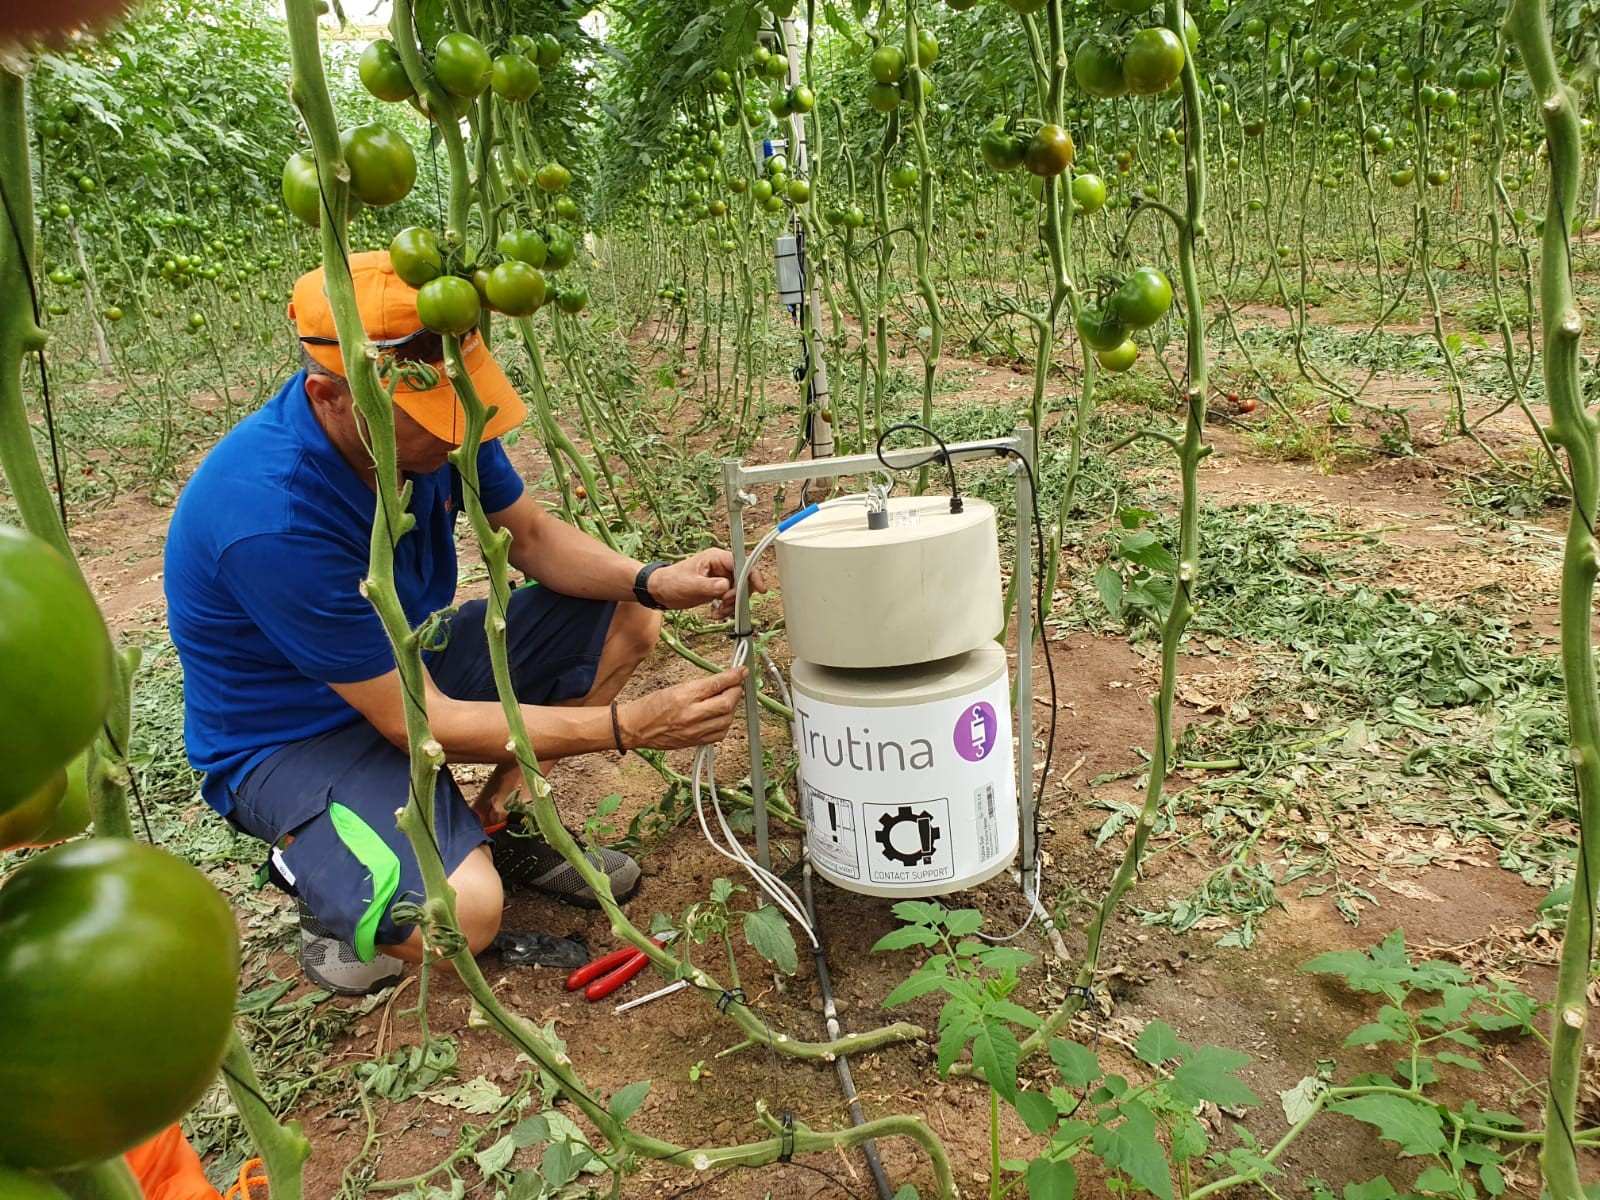
\includegraphics[width=10cm]{auto_water1.jpg}}
	\end{center}
	\caption{Trutina ~\cite{Trutina}}
\end{figure}


\newpage
\subsubsection{Arduino Irrigator System }

Ten projekt bazuje na płytce rozwojowej arduino UNO i ma na celu automatyzacje procesu pomiarów parametrów rośliny i jej podlewaniu. System czyta wilgotność gleby i włącza pompę wodną jeśli wilgotność spadnie poniżej pewnego poziomu. Kiedy system wykryje wartość powyżej ustalonej wyłączy pompę. System posiada także wyświetlacz LCD 16x2 na którym są wyświetlane: poziom wody w zbiorniku, status czy pompka jest włączona, wilgotność gleby.

Projekt różni się od naszego sposobem wyświetlania danych - różnica wyświetlaczy, a także brakiem zapisywania pomiarów i połączeniem z siecią Wi-Fi.



\begin{figure}[!h]
	\begin{center}
		{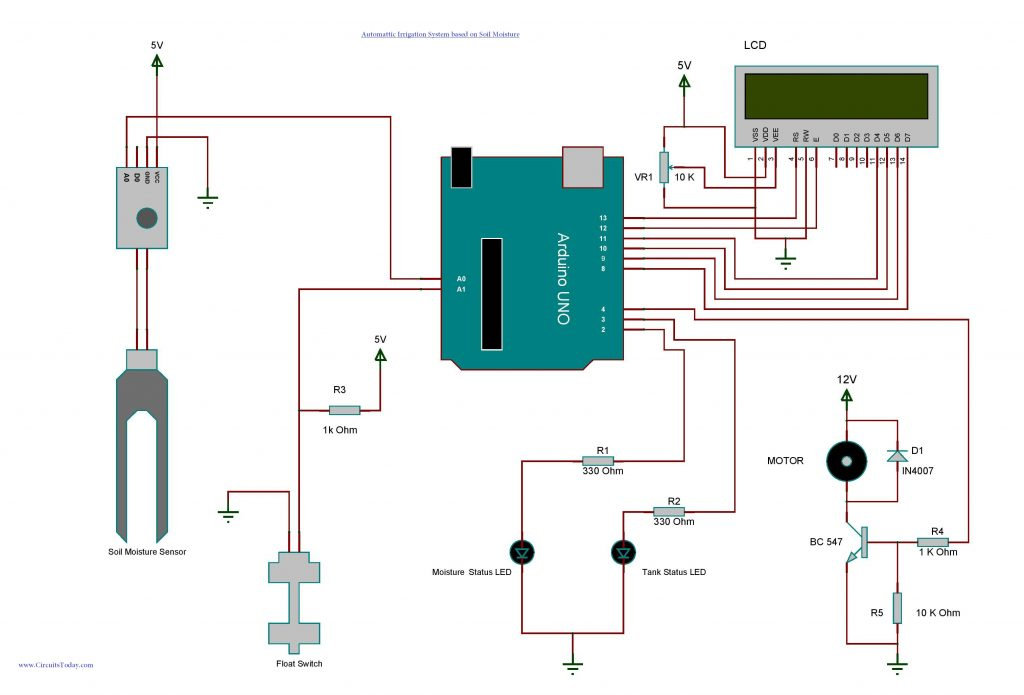
\includegraphics[width=8cm]{arduino_przyklad2.jpg}}
	\end{center}
	\caption{Arduino Irrigator System ~\cite{ArduinoIS}}
\end{figure}

\section{Szczegółowy opis projektu}


\subsection{Rozwiązania techniczne - Przegląd modułów projektu}
\subsubsection{Czujnik wilgotności i temperatury powietrza: DHT11}
Pomiary wilgotności i temperatury powietrza są wykonywane z użyciem czujnika DHT11. Do implementacji w ArduinoIDE została wykorzystana biblioteka DHT-sensor-library, aby pomiary wykonywały się poprawnie, dzięki czemu ręczna kalibracja nie była potrzebna.
\begin{figure}[!h]
	\begin{center}
		{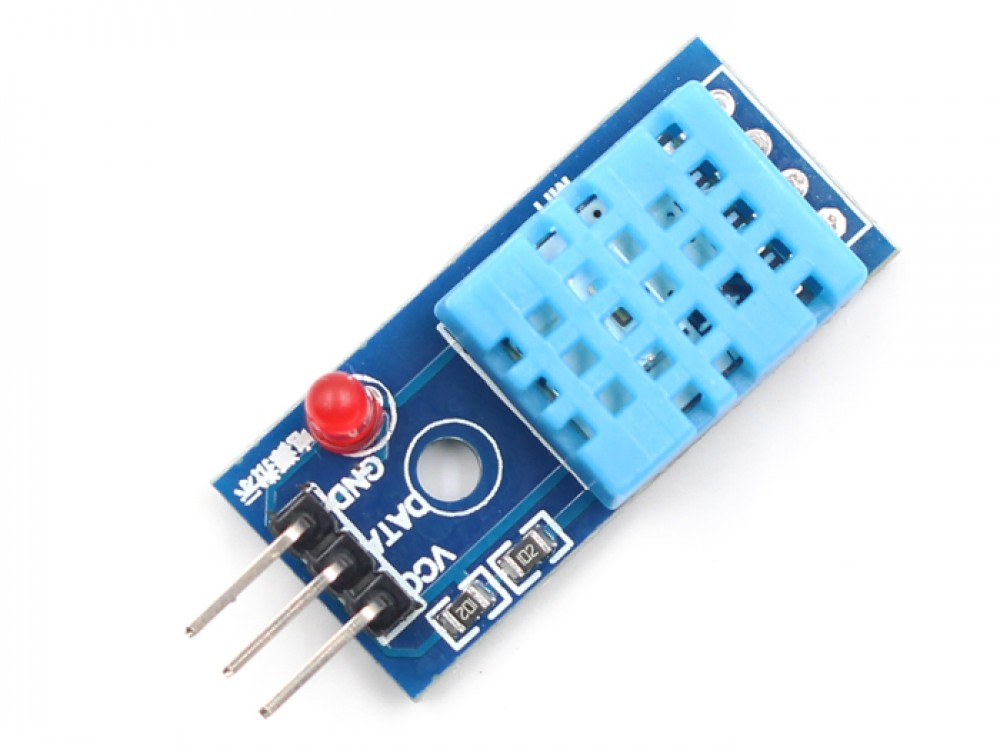
\includegraphics[width=5cm]{DHT11_photo.png}}
	\end{center}
	\caption{Czujnik DHT11}
\end{figure}


\newpage
\subsubsection{Czujnik natężenia światła}
Pomiary natężenia aktualnego oświetlenia w otoczeniu rośliny są wykonywane z użyciem czujnika natężenia światła. Jego parametry były skonfigurowane na podstawie własnych doświadczeń: 0 procent - czujnik zakryty ciemnym materiałem, 100 procent - czujnik oświecony mocnym źródłem światła.
\begin{figure}[!h]
	\begin{center}
		{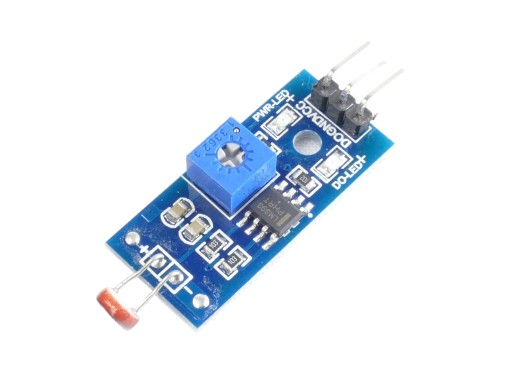
\includegraphics[width=7cm]{light_sensor_photo.png}}
	\end{center}
	\caption{Czujnik natężenia światła}
\end{figure}
\subsubsection{Czujnik wilgotności gleby FC-28}
Pomiary wilgotności gleby naszej rośliny są wykonywane z użyciem czujnika wilgotności gleby FC-28. Jego parametry były skonfigurowane na podstawie własnych doświadczeń: 0 procent - czujnik w powietrzu - brak powierzchni styku, 100 procent - czujnik zanurzony w wodzie.

\begin{figure}[!h]
	\begin{center}
		{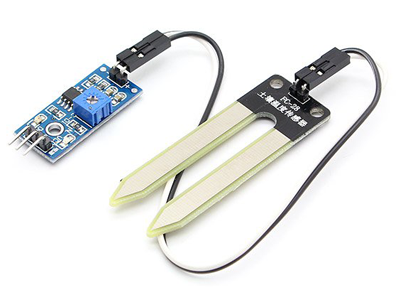
\includegraphics[width=7cm]{FC-28_photo.png}}
	\end{center}
	\caption{Czujnik FC-28}
\end{figure}

\newpage
\subsubsection{Czujnik poziomu wody w zbiorniku}
Pomiary aktualnego poziomu wody w zbiorniku z wodą do podlewania są wykonywane z użyciem czujnika poziomu wody. Jego parametry były skonfigurowane na podstawie własnych doświadczeń: 0 procent - czujnik suchy, nie zanurzony w wodzie, 100 procent - czujnik w całości zanurzony w wodzie.
\begin{figure}[!h]
	\begin{center}
		{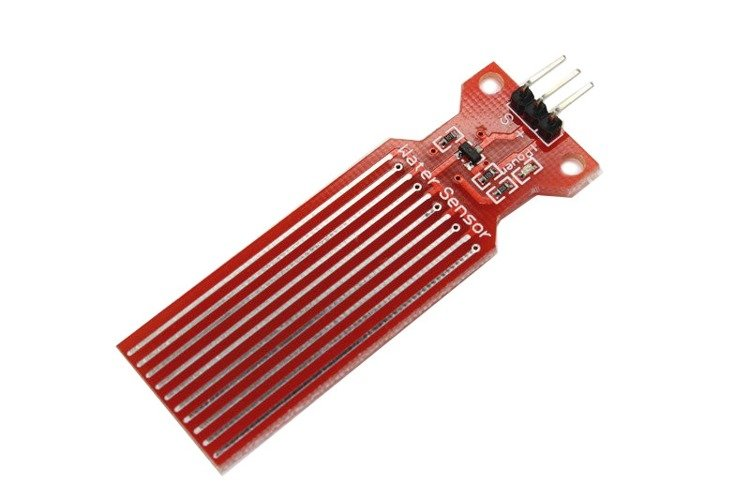
\includegraphics[width=6cm]{water_sensor_photo.png}}
	\end{center}
	\caption{Czujnik poziomu wody}
\end{figure}

\subsubsection{Wyświetlacz OLED}
Zewnętrzne wyświetlanie pomiarów wilgotności gleby i powietrza jest obsługiwane przez wyświetlacz OLED zamontowany na przodzie obudowy, aby była możliwość monitorowania jej stanu, gdy przebywamy w jej otoczeniu bez potrzeby połączenia internetowego. Do poprawnego wyświetlania danych na ekranie zostały wykorzystane biblioteki AdafruitGFX.h i AdafruitSSD1306.h.
\begin{figure}[!h]
	\begin{center}
		{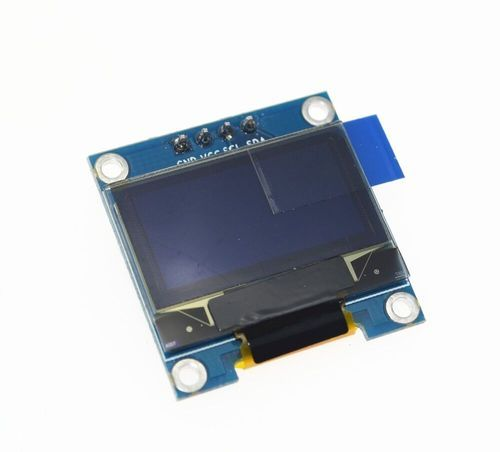
\includegraphics[width=8cm]{oled-display_photo.png}}
	\end{center}
	\caption{0.96 calowy wyświetlacz OLED}
\end{figure}

\subsubsection{Przekaźnik, Pompka wodna}
Do układu została zamontowana samochodowa pompka do spyskiwaczy firmy TOPRAN, gdyż było to tańsze rozwiązanie niż inne rodzaje pompek. Jej napięcie znamionowe wynosi 12 [V]. W projekcie do jej zasilania używamy baterii 9 [V]. Jej okresowe zasilanie jest realizowane za pomocą przekaźnika do którego z jednej strony wpięta jest bateria i pompka, a z drugiej zasilanie 5 [V] z płytki rozwojowej UNO, GND i sygnał sterujący.




\begin{figure}[!h]
%%obrazki
\centering
\subfloat[Przekaźnik~\cite{przekaznik}]{\label{odnosnik}
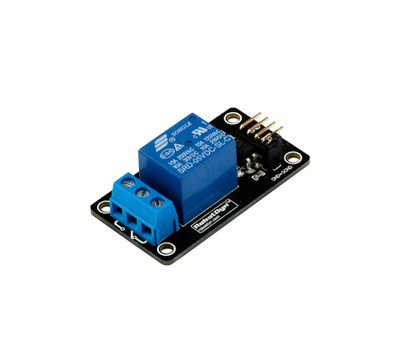
\includegraphics[width=0.4\textwidth]{Przekaznik_photo.jpg}}
\quad
\subfloat[Pompa wodna~\cite{pompka}]{\label{odnosnik}
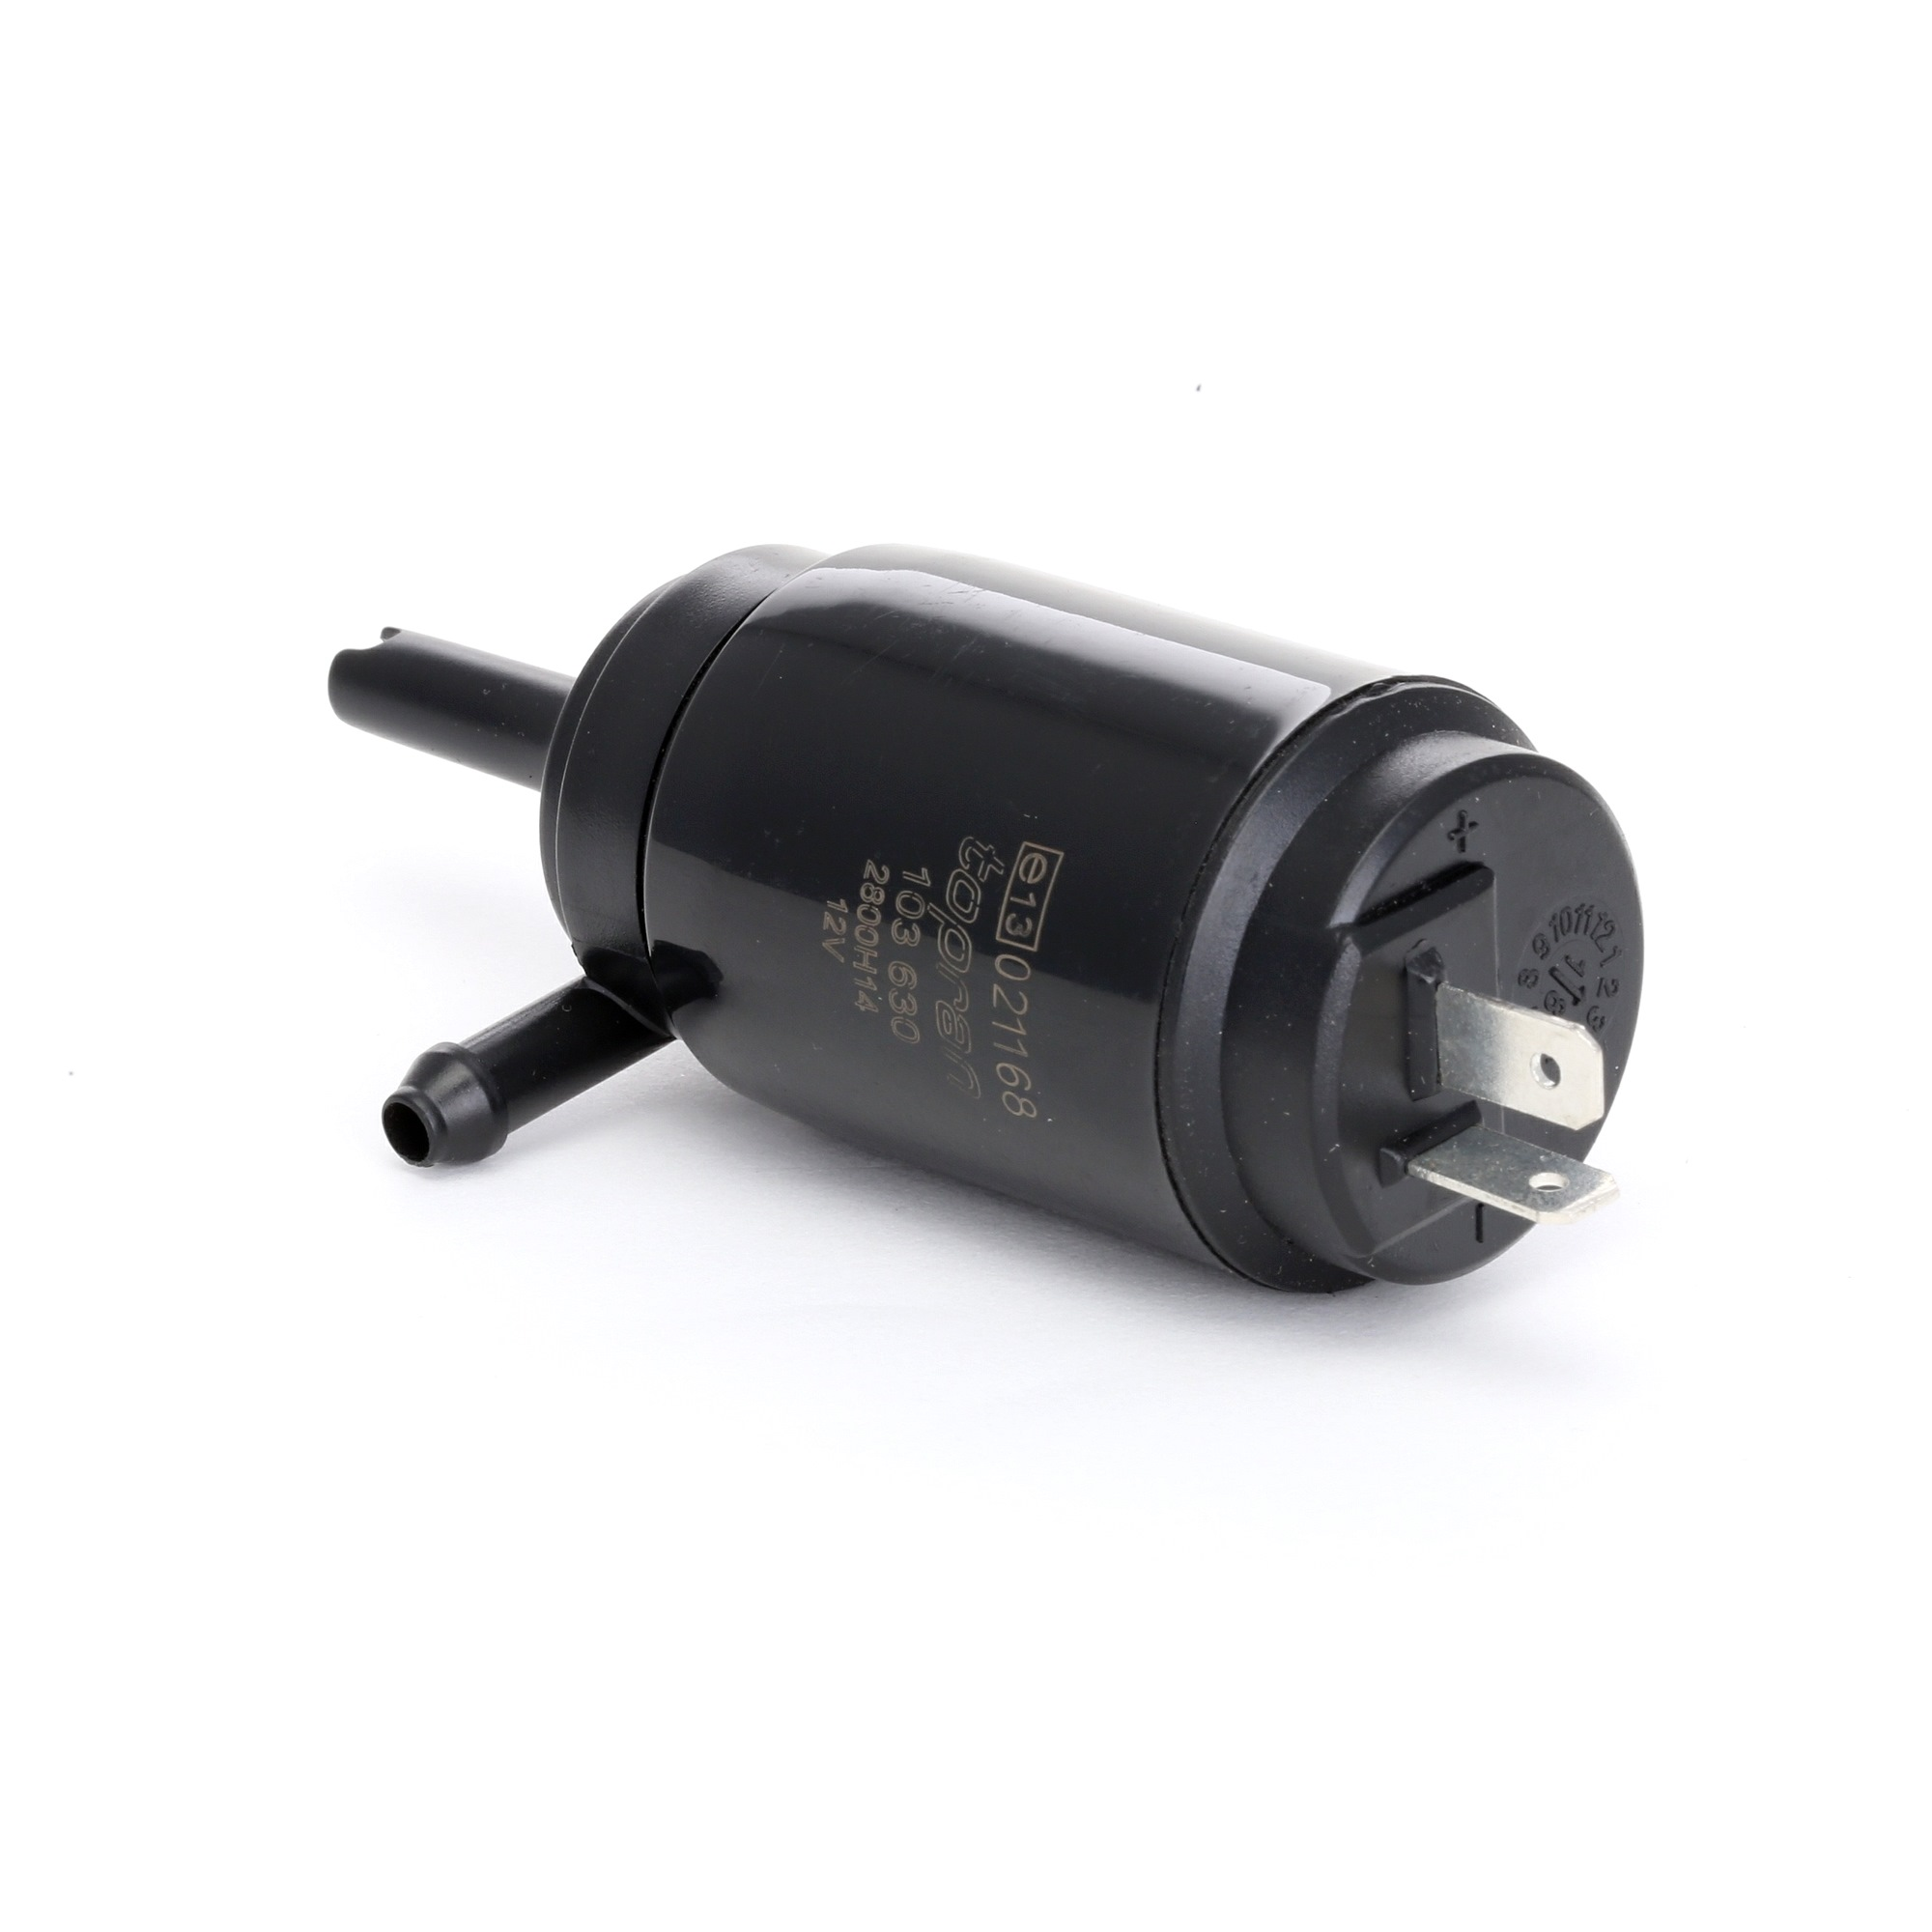
\includegraphics[width=0.4\textwidth]{pompka_photo.png}}
\quad
\subfloat[Bateria 9V~\cite{bateria}]{\label{odnosnik}

\includegraphics[width=0.4\textwidth]{9v.jpg}}
\caption{Komponenty pompki}

\end{figure}



\newpage
\subsubsection{Obudowa}
Obudowa na komponenty naszego projektu została zaprojektowana w programie Fusion360. Model ten został ''pocięty'' (przygotowany do druku) przy użyciu programu Cura i wydrukowany na drukarce 3D Ultimaker 2+. Został użyty materiał do drukowania o nazwie PLA (Polilaktyd) i dyszy wielkości 0.8mm. Czas drukowania pokrywki i pudełka wyniósł 12 godzin, nie licząc nieudanych druków i czasu spędzonego na dostrajanie drukarki.

\begin{figure}[!h]
	\begin{center}
		{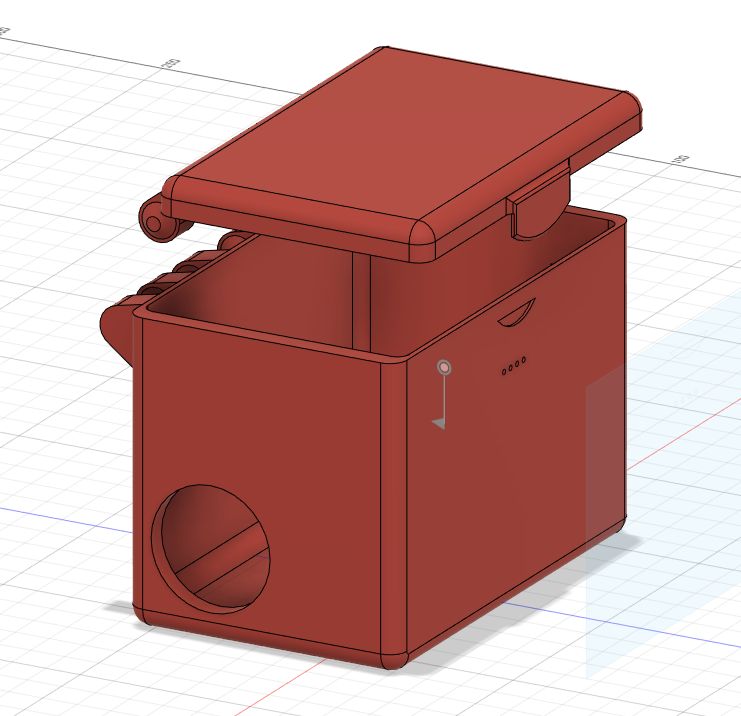
\includegraphics[width=9cm]{obudowa_model.png}}
	\end{center}
	\caption{Model obudowy (Fusion360)}
\end{figure}

\subsection{Szczególne rozwiązania warstwy programowej}
\subsubsection{Płytka rozwojowa UNO}
Realizacja oczekiwania płytki rozwojowej UNO na sygnał sterujący z ESP8266 została wykonana poprzez ciągłe sprawdzanie czy mamy coś w jej buforze. Gdy wykryjemy że jest coś do odczyania zczytujemy ten znak. Dane które są odbierane będą zawarte w wskaźnikach początku ''<'' i końca ''>'' danej komendy, dzięki temu możemy wykryć kiedy zaczyna się nowa instrukcja i wyczyścić pozostałości jakie mogły pozostać w buforze, a także wykryć zakończenie danej instrukcji. Zapobiega to "gubieniu danych" i otrzymywaniu powielonych instrukcji.
\begin{spverbatim}
	Część kodu płytki rozwojowej UNO odbierająca dane
\end{spverbatim}
\begin{lstlisting}
while (Serial.available()) 
{
	char serialChar = Serial.read(); 
	if (serialChar == '<')  
	{
		serialMessage = "";
		serialMessage += serialChar;
	}
	else if (serialChar == '>')
	{
		stringComplete = true;
		serialMessage += serialChar;
	}
	else
	{ 
		if ((serialChar >= 48 && serialChar <= 122) || serialChar == ',') 
		serialMessage += serialChar;
	}}
	if( stringComplete == true)
\end{lstlisting}


\begin{figure}[!h]
	\begin{center}
		{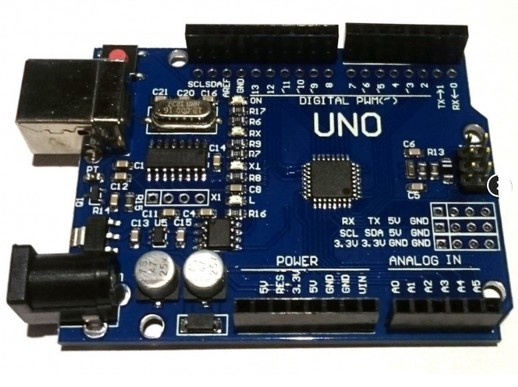
\includegraphics[width=12cm]{uno_photo.png}}
	\end{center}
	\caption{Płytka rozwojowa UNO}
\end{figure}

\subsubsection{ESP8266}
Połączenie płytki ESP8266 z Internetem jest realizowane z pomocą biblioteki ESP8266WiFi.h która ułatwia nam połączenie poprzez dodanie klasy WiFiClient, która przyjmując argumenty nazwy sieci Wi-Fi i hasła łączy się automatycznie z internetem.
Gdy już uzyskamy połączenie z siecią Wi-Fi łączymy się z naszym serwerem na wcześniej zadeklarowanym IP i porcie za pomocą metody stworzonej z użyciem biblioteki WebSocketClient.h.
Aby ułatwić testowanie po każdym nieudanym połaczeniu restertujemy ESP, aby próbowało cały czas się połączyć.

Tak jak w płytce rozwojowej UNO, odbieranie i wysyłanie danych jest realizowane we wskaźnikach początku ''<'' i końca ''>''.
\begin{figure}[!h]
	\begin{center}
		{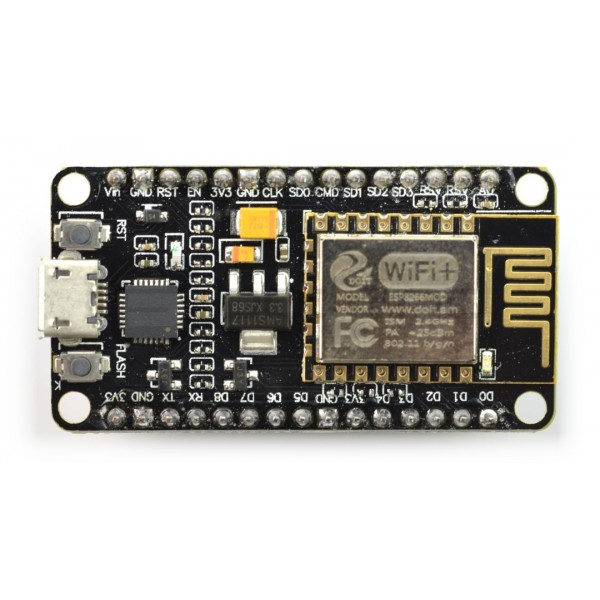
\includegraphics[width=12cm]{esp8266_photo.png}}
	\end{center}
	\caption{ESP8266}
\end{figure}
\subsubsection{Panel sterowania przez Internet}


\section{Realizacja projektu}
\subsection{Problematyka projektu}
Przed rozpoczęciem prac nad projektem utworzyliśmy tabele w programie internetowym Trello, na których zapisaliśmy rzeczy potrzebne do zrobienia, a także podział kto jaką cześcią projektu się zajmie. Najtrudniejszą częścią wydawała nam się implementacja połączeń pomiędzy płyką rozwojową UNO, ESP8266, a serwerem, więc postanowiliśmy zacząć od tego, a dopiero później przejść do następnych aspektów projektu. 

\subsection{Sposób wykonania}


Postanowiliśmy połączyć płytkę rozwojową UNO obsługującą pompkę i monitorującą wartości naszych czujników z ESP8266, aby była możliwość sterowania poprzez Internet.

Płytka rozwojowa UNO cały czas czeka na przychodzące dane które będą zawarte w wskaźnikach początku ''<'' i końca ''>'' danej komendy, aby wykonać określoną czynność lub odesłać pomiary wykonane przez czujnik wilgotności i temperatury do ESP8266, które jest połączone z UNO poprzez piny RX i TX. UNO odsyła swoje komendy również w wskaźnikach początku i końca, aby zapobiec ''gubieniu'' danych.

ESP8266 jest naszym tzw. ''mostem'' i w każdym momencie czeka na dane czy to z UNO czy ze strony internetowej i w zależności od kogo dane otrzymuje przerzuca je do danego odbiorcy.
Program na ESP jest zrealizowany z użyciem bibliotek ESP8266WiFi, WebSocketClient, SoftwareSerial, które kolejno służą do: umożliwieniu połączenia się ESP do sieci WiFi zadeklarowanej w naszym kodzie, połączeniu się poprzez websocket jako klient do naszego serwera postawionego na laptopie, połączenia się poprzez piny RX i TX do płytki rozwojowej UNO.

\subsection{Problemy napotkane podczas realizacji}
\subsubsection{Połączenie między UNO, a ESP8266}
Próbowaliśmy różnych typów połączeń jak I2C, albo SPI jednak poprawność testowych danych jakie otrzymywaliśmy była nikła - albo dostawaliśmy tylko cześć danych albo były one w różny sposób powielone.
Rozwiazaliśmy ten problem poprzez użycie wskaźników początku ''<'' i końca ''>'' przy wysyłaniu danej komendy, aby wykonać określoną czynność lub odesłać pomiary. 
\subsubsection{Projektowanie i drukowanie obudowy}
Dużym problemem była niewiedza związana z wielkością jaką powinna mieć obudowa, jednak zdecydowaliśmy że będzie ona większa niż będziemy potrzebować, aby umożliwić nam łatwe rozbudowanie projektu w przyszłości. 


\begin{figure}[!h]
	\begin{center}
		{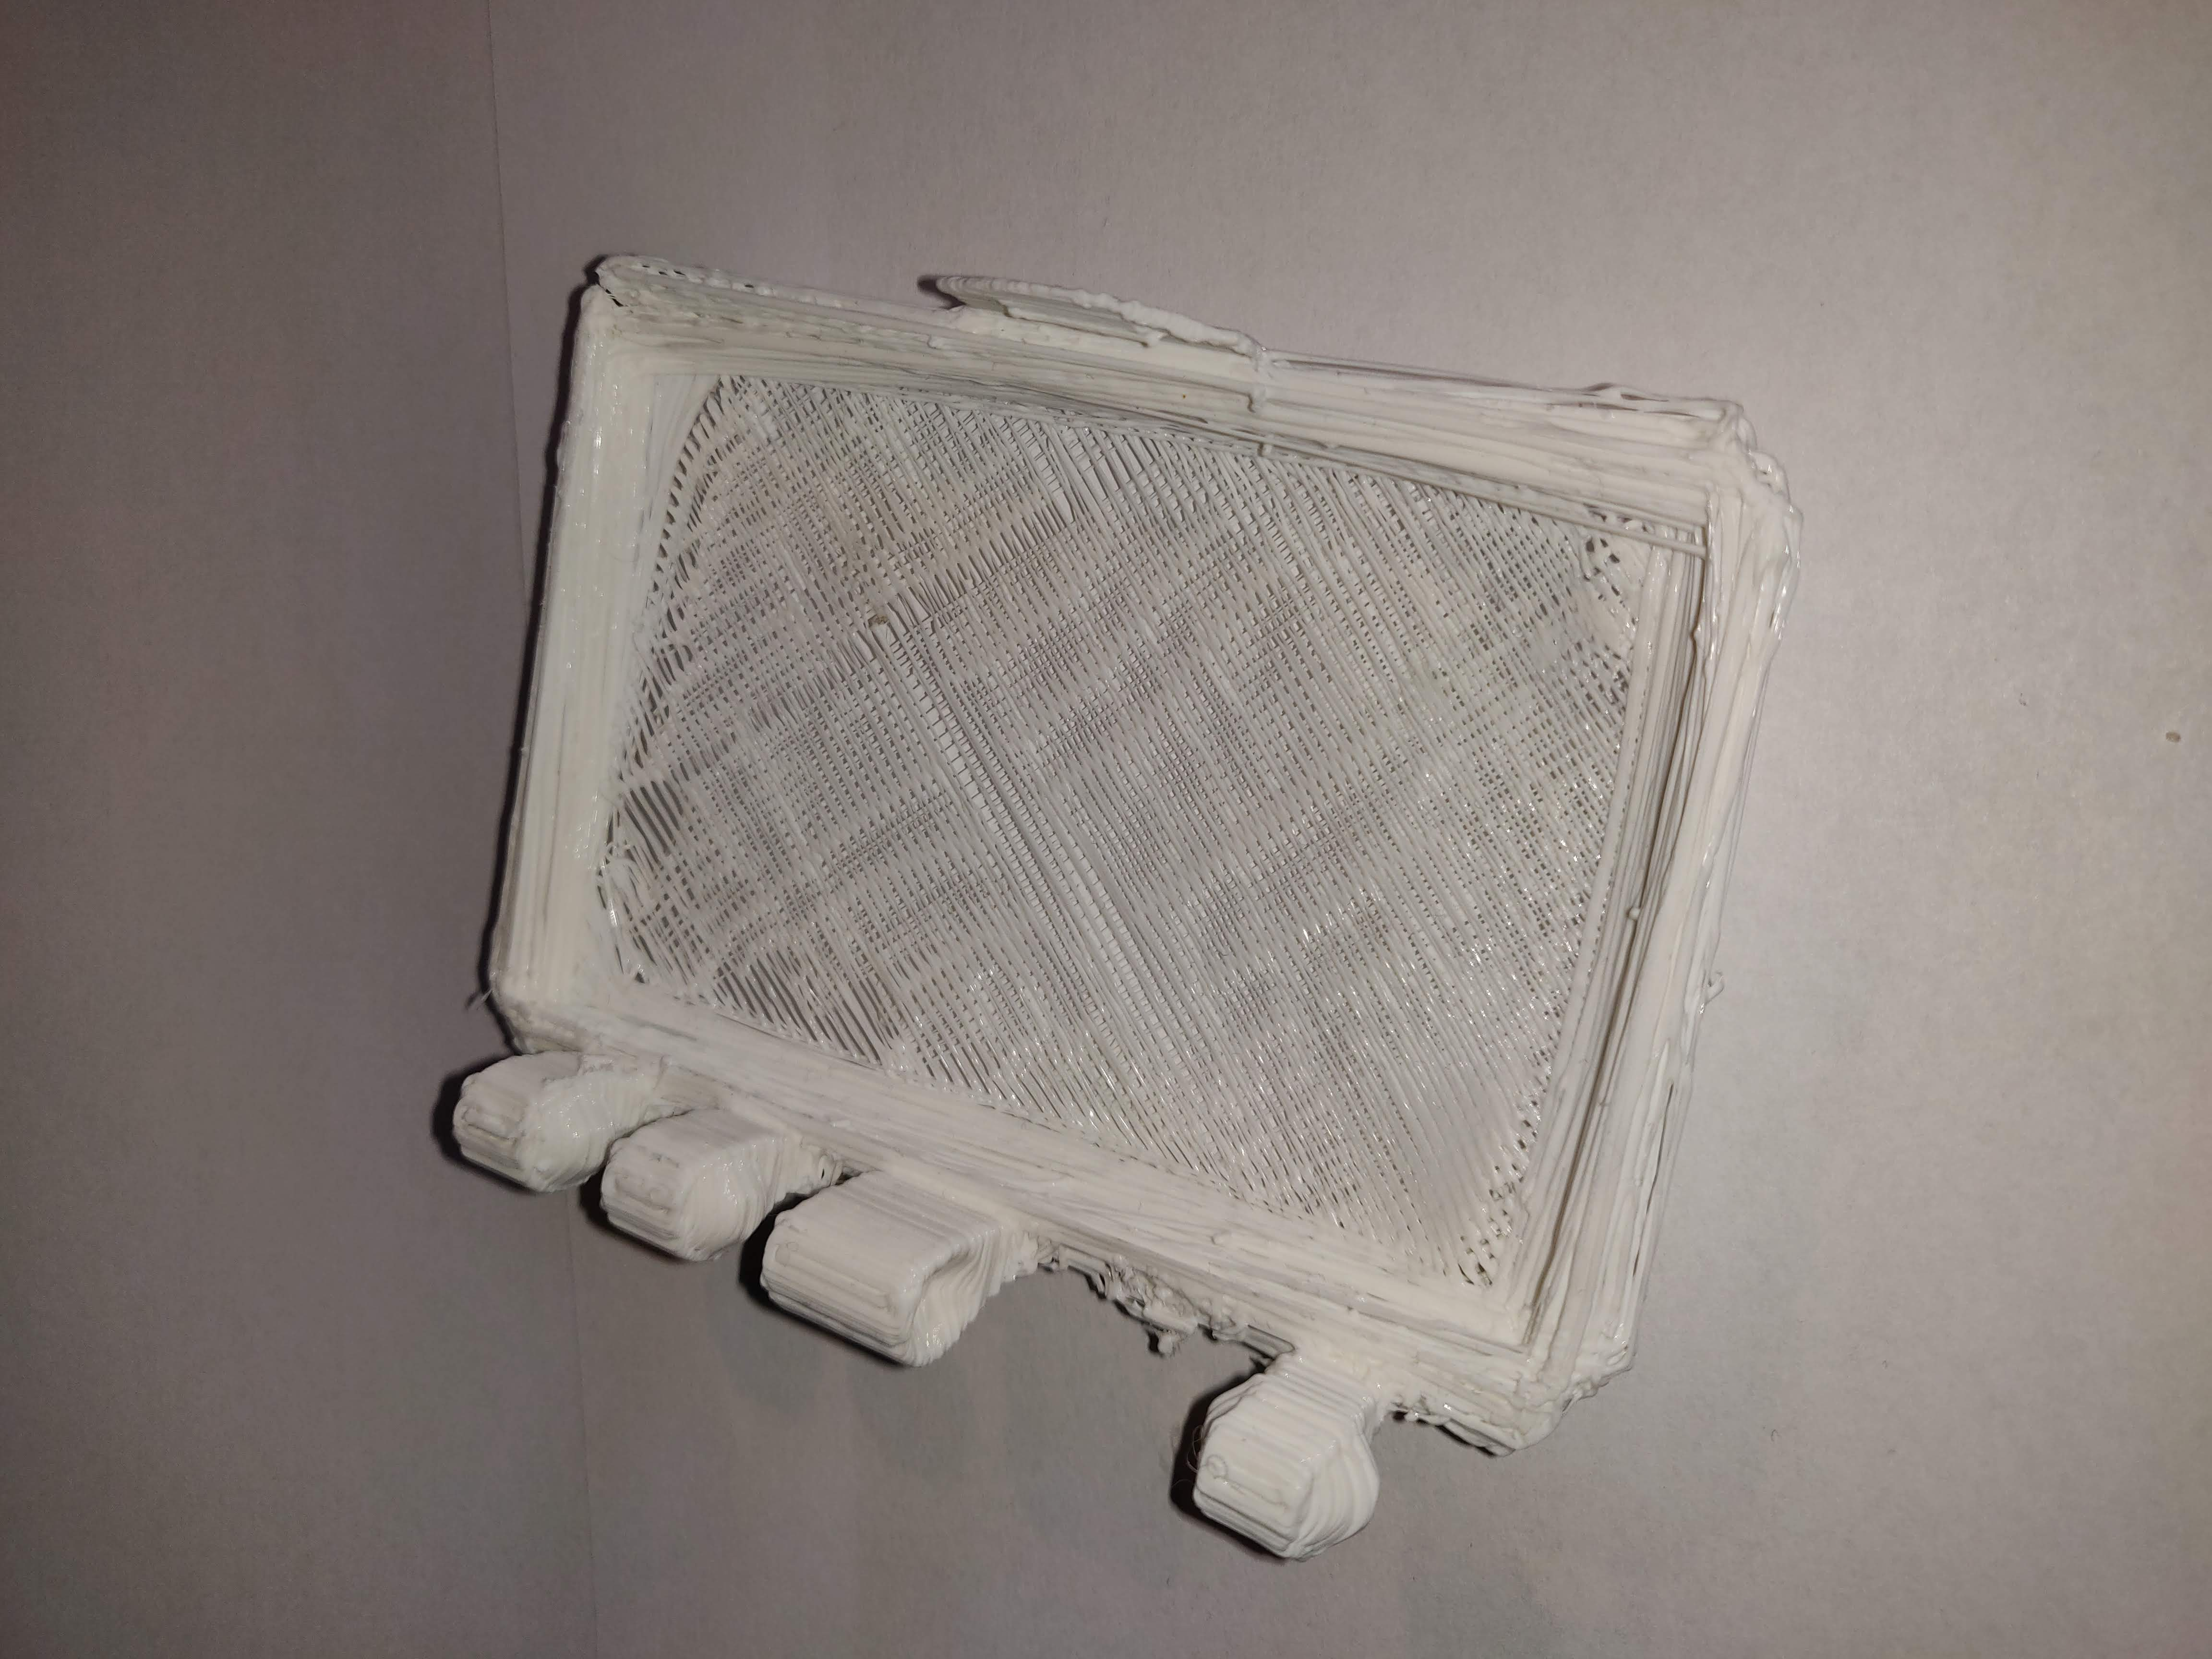
\includegraphics[width=12cm]{obudowa_broken.jpg}}
	\end{center}
	\caption{Nieudany druk pokrywki}
\end{figure}

Przy początkach drukowania popełniliśmy błąd złej początkowej wysokości druku co spowodowało że model był drukowany w powietrzu a co za tym idzie druk się nie powiódł. Kalibracja drukarki 3D naprawiła nasz problem i druk został wykonany poprawnie



\section{Harmonogram i podział obowiązków}

\subsection{Podział obowiązków}

\subsection{Wstępny schemat blokowy}
Przed rozpoczęciem pracy nad projektem stworzyliśmy schemat, którego staraliśmy się trzymać jednak ze względu na pewne komplikacje w trakcie realizacji pewne aspekty zostały zmienione co zostało przedstawione na finalnym schemacie blokowym.
\begin{figure}[!h]
	\begin{center}
		{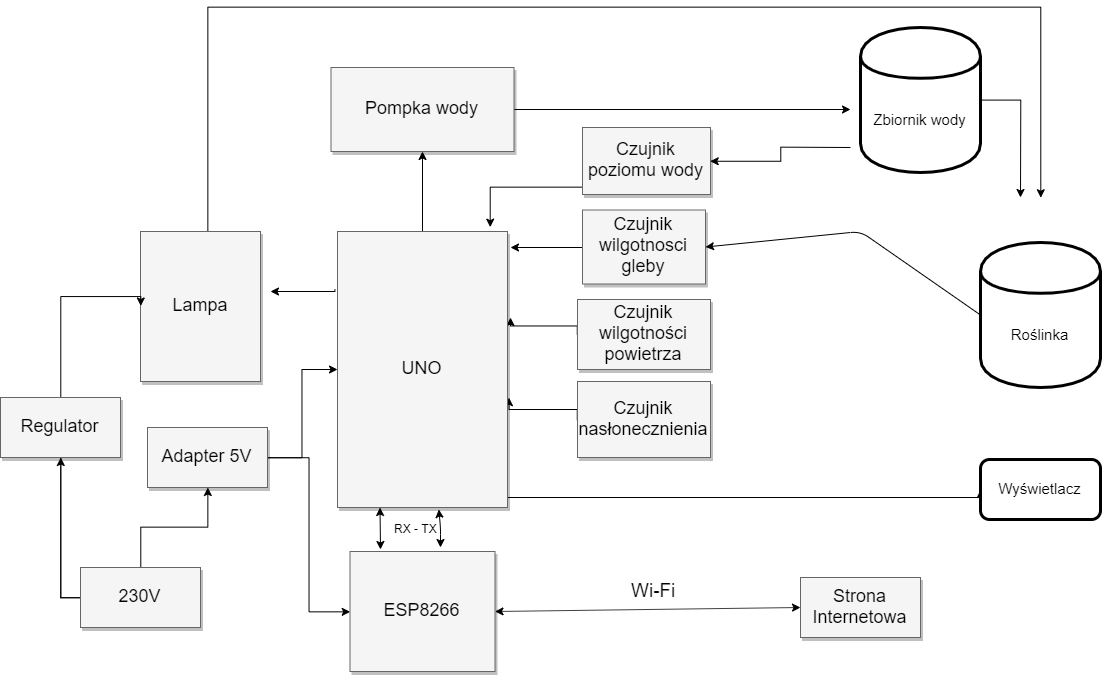
\includegraphics[width=16cm]{schemat_blokowy.png}}
	\end{center}
	\caption{Wstępny schemat blokowy}
\end{figure}

\subsection{Harmonogram}
\subsubsection{4.11}
Przeanalizowanie schematów płytki rozwojowej UNO, modułu komunikacyjnego ESP8266, czujnika wilgotności gleby, czujnika wilgotności powietrza, czujnika nasłonecznienia oraz rozwiązanie techniczne doświetlania rośliny. Stworzenie schematu elektrycznego gotowego projektu. Testowanie poprawności działania posiadanych czujników w warunkach domowych. Implementacja komunikacji z modułem ESP8266. Dopasowywanie czasów działania. 
Dokupienie brakujących komponentów gotowego projektu. 
\subsubsection{25.11}
Realizacja połączeń elektrycznych na płytce stykowej i ostateczne testowanie poprawności dzia-
łania. Przeniesienie projektu na płytkę uniwersalną. Przygotowanie ewentualnej obudowy i realiza-
cja montażu systemu doświetlania. Stworzenie prezentacji na zajęcia

\subsubsection{16.12}
Wstępna prezentacja gotowego projektu i ocena błędów.

\subsubsection{20.01}
Ostateczna prezentacja z poprawką błędów.



\subsection{Zgodność z harmonogramem}
Okazało się że założony harmonogram był zbyt optymistyczny, założyliśmy za dużo rzeczy do zrobienia w początkowej części harmonogramu, a nie ustaliliśmy dużo na końcową część. Jednak dzięki temu mieliśmy czas na dokończenie zaplanowanych aspektów projektu i nie przekroczeniu danego czasu na ukończenie projektu.

\subsubsection{4.11}
Rozpoczęliśmy prace nad naszym projektem. Postanowiliśmy skorzystać z aplikacji internetowej Trello do utworzenia tabel, które pozwoliły by nam na lepsze zarządzanie podziałem prac nad projektem.

Przeanalizowaliśmy schematy płytki rozwojowej UNO, modułu komunikacyjnego ESP8266, czujnika wilgotności gleby, czujnika wilgotności powietrza oraz czujnika nasłonecznienia. Przeanalizowaliśmy działanie każdego z czujników poprzez wykonanie przykładowych kodów na płytce rozwojowej UNO. Dowiedzieliśmy się jakich komponentów projektu nam brakuje i zamówiliśmy je w wybranych sklepach.
Stworzyliśmy wstępny schemat blokowy projektu, aby ukazać działanie poszczególnych elementów zawartych w naszym projekcie. Na ten moment postanowiliśmy nie tworzyć schematu elektrycznego, gdyż nie wiedzieliśmy jak dokładnie zrealizujemy poszczególne połączenia.

Ze względu na obszerność testowania i planowanie realizacji planu działania na nadchodzące tygodnie nie zajęliśmy się komunikacją z modułem ESP8266, ani problemem związanym z doświetlaniem naszej rośliny.


\subsubsection{25.11}
Do tego dnia zajmowaliśmy się komunikacją między płytką rozwojową UNO, ESP8266, a stroną internetową. Napotkaliśmy wiele problemów co nieplanowanie wydłużyło nam pracę na tym etapie projektu. Udało nam się uzyskać stabilne połączenie między naszymi urządzeniami. Zrealizowaliśmy połączenia UNO, ESP8266, a także podłączyliśmy do układu czujnik wilgotności i temperatury powietrza i na płytce stykowej po czym przetestowaliśmy poprawność działania. 

Przeniesienie projektu na płytkę uniwersalną okazało się niepraktyczne na tym etapie projektu, gdyż nie próbowaliśmy jeszcze połączyć ze sobą wszystkich modułów projektu i finalny kod do wgrania na UNO i ESP8266 nie był gotowy. Z powodu niewiedzy jak dokładnie będzie wyglądało nasze urządzenie na płytce uniwersalnej nie przygotowaliśmy planowanej obudowy. Nie zrealizowaliśmy również systemu doświetlania.

\subsubsection{16.12}
Podłączyliśmy ze sobą wszystkie czujniki na płytce uniwersalnej i testowaliśmy poprawność działania. Zajęliśmy się projektowaniem obudowy w programie Fusion360, abyśmy mogli ją wydrukować na drukarce 3D i włożyć do obudowy komponenty naszego projektu. Wydrukowaliśmy obudowę i wsadziliśmy tam wszystkie moduły projektu.

\subsubsection{20.01}
Ostateczna prezentacja.



\section{Podsumowanie }
\subsection{Osiągnięte cele}
To our surprise, the project in general was more time consuming that we could ever expect. The lack of knowledge makes it hard to even get one, because we did not really know what to look for. Thankfully, the Internet nowadays provides lots of resources and tutorials that helped us in comming up with solutions and finding out why they do not work. In conclusion we are proud of the outcome, not everything went as expected but we managed to combine software and hardware solutions and make them work together. 
The project forced us to think outside of the box as there were neither imposed technologies nor the way to write our code. It was good practise to come up with something of our own, develop that one idea and bring it to the end.
\subsection{Pomysły na rozwój projektu}
Automatyzacja procesu podlewania
Aplikacja
Domena i działanie projektu w chmurze bez potrzeby włączania serwera na laptopie. Do tego było by potrzebne przeniesienie naszej bazy danych na bazę danych w chmurze (np. Azure), a także implementacja ESP8266 jako serwera.
\begin{thebibliography}{9}



\bibitem{Trutina} Trutina z Gremon Systems
gremonsystems.com/blog-en/things-you-didnt-know-about-automatic-watering-systems/

\bibitem{ArduinoIS} Arduino Irrigator System
http://www.circuitstoday.com/arduino-irrigation-plant-watering-using-soil-moisture-sensor


\bibitem{latexcompanion} 
Michel Goossens, Frank Mittelbach, and Alexander Samarin. 
\textit{The \LaTeX\ Companion}. 
Addison-Wesley, Reading, Massachusetts, 1993.

\bibitem{latexcompanion} 
Ivan Grokhotkov
\textit{ESP8266 Arduino Core’s documentation}. 
2017

\bibitem{latexcompanion} 
Christian Klippel, Peter Andersson, Peter Lerup
\textit{ESP8266 core for Arduino}. 
2017

\bibitem{latexcompanion} 
guy
\textit{w3schools.com}. 
1999-2019
 
\bibitem{einstein} 
Albert Einstein. 
\textit{Zur Elektrodynamik bewegter K{\"o}rper}. (German) 
[\textit{On the electrodynamics of moving bodies}]. 
Annalen der Physik, 322(10):891–921, 1905.

\bibitem{przekaznik} Relay Module
\emph{},
opencircuit.shop/Product/Relay-Module-1-relay.-5V

\bibitem{pompka} Pompa spryskiwacza TOPRAN
\emph{},
www.autoczescionline24.pl/topran-2723484.html



\bibitem{bateria} Bateria alkaliczna 9V 
\emph{VARTA},
www.elfadistrelec.pl/pl/alkaliczne-bateria-alkaliczna-9v-6lr61-varta-industrial-9v/p/16901614



 
\bibitem{knuthwebsite} 
Knuth: Computers and Typesetting,
\\\texttt{http://www-cs-faculty.stanford.edu/\~{}uno/abcde.html}
\end{thebibliography}


\end{document}
